% Options for packages loaded elsewhere
\PassOptionsToPackage{unicode}{hyperref}
\PassOptionsToPackage{hyphens}{url}
%
\documentclass[
]{article}
\usepackage{amsmath,amssymb}
\usepackage{iftex}
\ifPDFTeX
  \usepackage[T1]{fontenc}
  \usepackage[utf8]{inputenc}
  \usepackage{textcomp} % provide euro and other symbols
\else % if luatex or xetex
  \usepackage{unicode-math} % this also loads fontspec
  \defaultfontfeatures{Scale=MatchLowercase}
  \defaultfontfeatures[\rmfamily]{Ligatures=TeX,Scale=1}
\fi
\usepackage{lmodern}
\ifPDFTeX\else
  % xetex/luatex font selection
\fi
% Use upquote if available, for straight quotes in verbatim environments
\IfFileExists{upquote.sty}{\usepackage{upquote}}{}
\IfFileExists{microtype.sty}{% use microtype if available
  \usepackage[]{microtype}
  \UseMicrotypeSet[protrusion]{basicmath} % disable protrusion for tt fonts
}{}
\makeatletter
\@ifundefined{KOMAClassName}{% if non-KOMA class
  \IfFileExists{parskip.sty}{%
    \usepackage{parskip}
  }{% else
    \setlength{\parindent}{0pt}
    \setlength{\parskip}{6pt plus 2pt minus 1pt}}
}{% if KOMA class
  \KOMAoptions{parskip=half}}
\makeatother
\usepackage{xcolor}
\usepackage[margin=1in]{geometry}
\usepackage{longtable,booktabs,array}
\usepackage{calc} % for calculating minipage widths
% Correct order of tables after \paragraph or \subparagraph
\usepackage{etoolbox}
\makeatletter
\patchcmd\longtable{\par}{\if@noskipsec\mbox{}\fi\par}{}{}
\makeatother
% Allow footnotes in longtable head/foot
\IfFileExists{footnotehyper.sty}{\usepackage{footnotehyper}}{\usepackage{footnote}}
\makesavenoteenv{longtable}
\usepackage{graphicx}
\makeatletter
\def\maxwidth{\ifdim\Gin@nat@width>\linewidth\linewidth\else\Gin@nat@width\fi}
\def\maxheight{\ifdim\Gin@nat@height>\textheight\textheight\else\Gin@nat@height\fi}
\makeatother
% Scale images if necessary, so that they will not overflow the page
% margins by default, and it is still possible to overwrite the defaults
% using explicit options in \includegraphics[width, height, ...]{}
\setkeys{Gin}{width=\maxwidth,height=\maxheight,keepaspectratio}
% Set default figure placement to htbp
\makeatletter
\def\fps@figure{htbp}
\makeatother
\setlength{\emergencystretch}{3em} % prevent overfull lines
\providecommand{\tightlist}{%
  \setlength{\itemsep}{0pt}\setlength{\parskip}{0pt}}
\setcounter{secnumdepth}{-\maxdimen} % remove section numbering
\ifLuaTeX
  \usepackage{selnolig}  % disable illegal ligatures
\fi
\usepackage{bookmark}
\IfFileExists{xurl.sty}{\usepackage{xurl}}{} % add URL line breaks if available
\urlstyle{same}
\hypersetup{
  pdftitle={Figures for Ekanayake-Weber et al.~2026},
  hidelinks,
  pdfcreator={LaTeX via pandoc}}

\title{Figures for Ekanayake-Weber et al.~2026}
\author{}
\date{\vspace{-2.5em}2025-12-12}

\begin{document}
\maketitle

This is an R Markdown document for easy access to and recreation of the
figures for the manuscript ``More Mouths to Feed?'', which is in prep
for submission to the journal PNAS.

There is first a setup chunk which loads the appropriate packages and
data.

\section{Main Text Tables and
Figures}\label{main-text-tables-and-figures}

\textbf{Table 1.} Most influential parameters, parameter ranges, and
parameter values when held constant.

\begin{longtable}[]{@{}
  >{\raggedright\arraybackslash}p{(\columnwidth - 8\tabcolsep) * \real{0.2000}}
  >{\raggedright\arraybackslash}p{(\columnwidth - 8\tabcolsep) * \real{0.2000}}
  >{\raggedright\arraybackslash}p{(\columnwidth - 8\tabcolsep) * \real{0.2000}}
  >{\raggedright\arraybackslash}p{(\columnwidth - 8\tabcolsep) * \real{0.2000}}
  >{\raggedright\arraybackslash}p{(\columnwidth - 8\tabcolsep) * \real{0.2000}}@{}}
\toprule\noalign{}
\begin{minipage}[b]{\linewidth}\raggedright
Parameter
\end{minipage} & \begin{minipage}[b]{\linewidth}\raggedright
Variable Name in NetLogo
\end{minipage} & \begin{minipage}[b]{\linewidth}\raggedright
Range for Global Sensitivity Analysis
\end{minipage} & \begin{minipage}[b]{\linewidth}\raggedright
Setting(s) for experiment to address H2
\end{minipage} & \begin{minipage}[b]{\linewidth}\raggedright
Setting(s) for experiment to address H3
\end{minipage} \\
\midrule\noalign{}
\endhead
\bottomrule\noalign{}
\endlastfoot
Clump size & clump-size & 1-500 & 1, 63, 126, 251, 376, 501 & 250 \\
Abundance & abundance & 200,000 - 1,200,000 & 200,000 to 1,200,000 in
steps of 225,000 & 600,000 \\
Energy per capita & energy-per-capita & 4,000 - 9,000 & 4,000 to 9,000
in steps of 1250 & 6,500 \\
Patch regrowth interval & patch-regrowth-interval & 500 - 2500 & 1000 &
1000 \\
Extraction rate mean & extraction-rate-mean & 2 - 8 & 5 & 5 \\
Target distance & tgt-dist & 1 - 40 & 1, 11, 21, 31, 41 & 1 to 41 in
steps of 4 \\
Target neighbors & tgt-neighbors & 3 - 11 & 3, 5, 7, 9, 11 & 3 - 11 \\
\end{longtable}

\begin{center}\rule{0.5\linewidth}{0.5pt}\end{center}

\begin{figure}
\centering
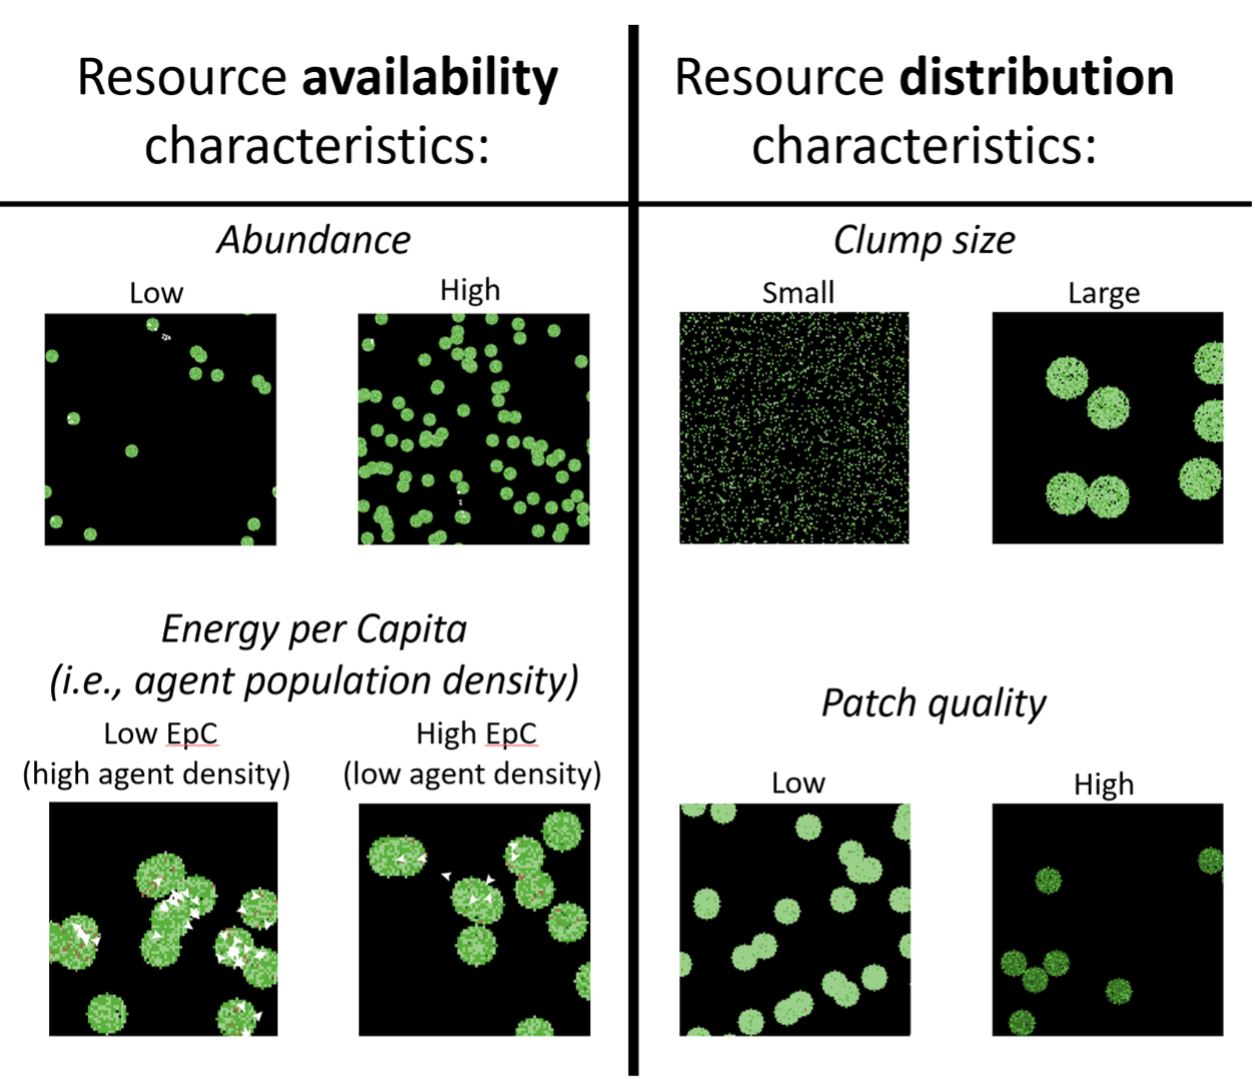
\includegraphics[width=\textwidth,height=0.05\textheight]{images/Figure1.png}
\caption{\textbf{Figure 1.} Illustration of the two major categories of
food resource characteristics, availability (left) and distribution
(right). For demonstration of each parameterized characteristic, all
other resource parameters are held constant. For example, when
increasing patch quality (lower right), the same amount of calories are
available on the landscape, but concentrated in fewer resource patches.
Rather than controlling resources directly, energy per capita (EpC,
lower left) determines the size of the agent population relative to the
amount of calories on the landscape.}
\end{figure}

\begin{center}\rule{0.5\linewidth}{0.5pt}\end{center}

\begin{figure}
\centering
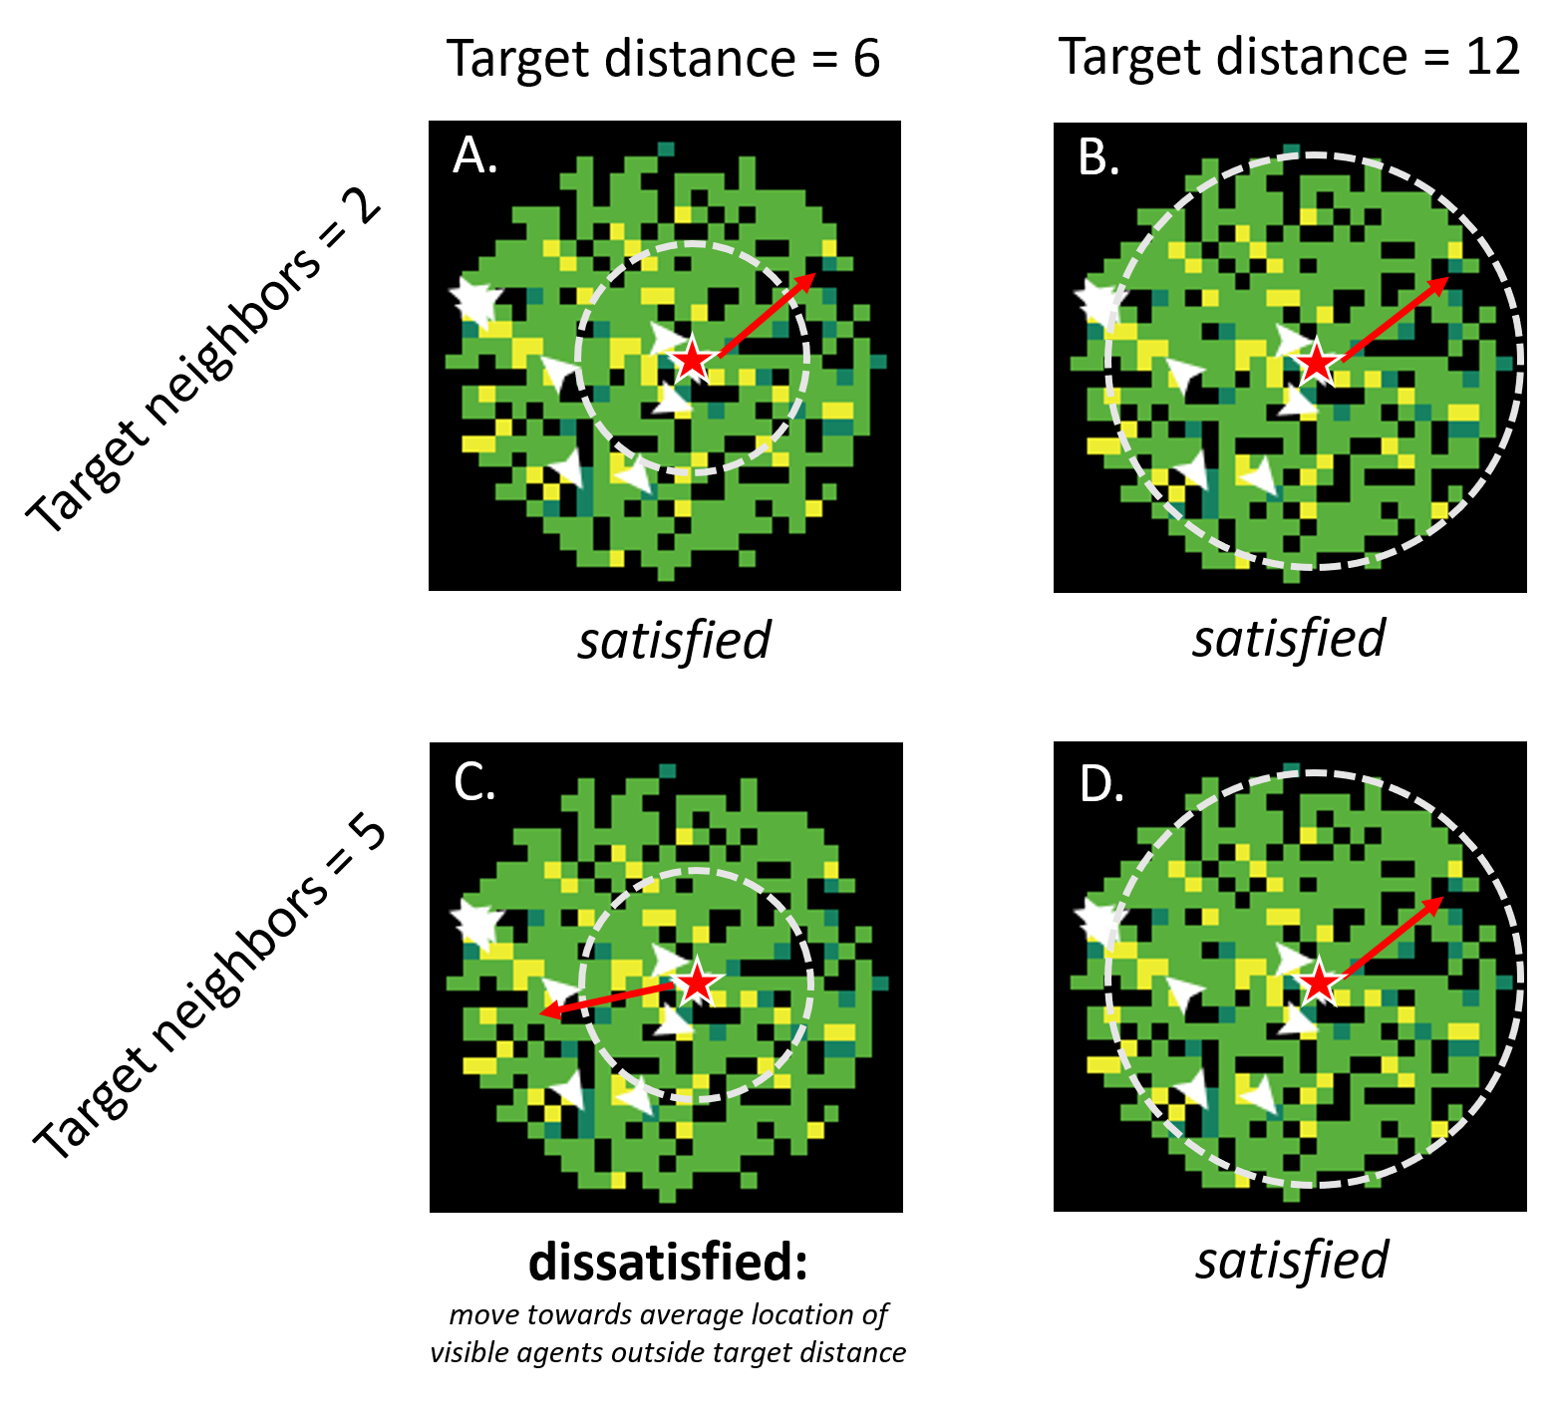
\includegraphics[width=\textwidth,height=0.05\textheight]{images/Figure2.png}
\caption{\textbf{Figure 2.} How the gregariousness rules worked in the
model using the two parameters, target distance and target neighbors.
Sensory range covers the entire square for all scenarios. Green and
yellow squares are resource patches of high and low energy contents,
respectively; black squares are empty patches. The red star is the
perspective agent; the white arrowheads are the non-perspective agents.
The white dashed line indicates the area with target distance of the
perspective agent. The red arrow represents the new heading of the
perspective agent. Agents would orient themselves towards the best
visible resource patch unless they did not have enough other agents
within target distance of themselves. In the left column (A, C), target
distance is 6. In the right column (B, D), target distance is 12. In the
upper row (A, B), target neighbors is 2. In the lower row (C, D), target
neighbors is 5. In A, B, and D, the perspective agent has satisfied
gregariousness rules, and will orient towards the highest-energy
resource patch. In C, the gregariousness rules are not satisfied, so the
perspective agent will orient towards any visible agents farther away
than target distance.}
\end{figure}

\begin{center}\rule{0.5\linewidth}{0.5pt}\end{center}

\begin{verbatim}
## [1] "Mean group size:  13.4482859622658"
\end{verbatim}

\begin{verbatim}
## [1] "Median group size:  10.1458333333333"
\end{verbatim}

\includegraphics{figureCode_files/figure-latex/figure3-1.pdf}

\textbf{Figure 3.} Distribution of and major resource influences on
population mean group size. \textbf{A.,} the distribution of mean group
sizes produced by the model across the primate-relevant parameter space.
The x-axis (group size) is on a log10 scale. Grand mean group size was
13.45 (median 10.15). \textbf{B., C., and D.,} heatmaps showing
interactions of the three most influential resource parameters on mean
group size. Each cell represents the mean outcome of 5 simulation
replicates. Simulations used to produce these heatmaps had all other
parameters held constant. In \textbf{B. and D.,} energy abundance is
divided by 1000 for display purposes. Mean group size tended to be
higher when clumps were large, abundance was low, and/or energy per
capita was low.

\begin{center}\rule{0.5\linewidth}{0.5pt}\end{center}

\includegraphics{figureCode_files/figure-latex/figure4-1.pdf}

\textbf{Figure 4.} Relationships between population mean group size and
population mean energy intake rate, for clump sizes ranging from 1 to
501 (A), and separated for small (B), medium (C), and large (D) clumps.
Resource abundance, energy per capita, and gregariousness were also
allowed to vary, but all other parameters were held constant. Each dot
represents a population mean of a single simulation. Each line
corresponds to a linear regression, with formulae (using the log10 group
size) displayed on each plot. A. when clump size was 1. B. when clump
size was 1. C. when clump size was 126. D. when clump size was 501.

\begin{center}\rule{0.5\linewidth}{0.5pt}\end{center}

\includegraphics{figureCode_files/figure-latex/figure5-1.pdf}

\textbf{Figure 5.} Relationships between population mean group size and
population mean daily travel distance, for clump sizes ranging from 1 to
501 (A), and separated for small (B), medium (C), and large (D) clumps.
Resource abundance, energy per capita, and gregariousness were also
allowed to vary, but all other parameters were held constant. Each dot
represents a population mean of a single simulation. Each line
corresponds to a linear regression, with formulae (using the log10 group
size) displayed on each plot. A. all clump sizes (1 to 501) combined .
B. when clump size was 1. C. when clump size was 126. D. when clump size
was 501.

\begin{center}\rule{0.5\linewidth}{0.5pt}\end{center}

\includegraphics{figureCode_files/figure-latex/figure6-1.pdf}

\textbf{Figure 6.} The relationship between group size and foraging
efficiency, mediated by the maximum distance that agents would tolerate
being from group members (``target distance''). The number of group
members that each agent attempted to keep in proximity (``target
neighbors'') was also allowed to vary across these simulations. Each dot
represents a population mean of a single simulation. The black lines are
linear regressions for each category of target distance. Formulae for
the regression lines (using the log group size) are displayed on each
plot. \textbf{A.} when target distance was less than 20, which meant
that agents maintained closer proximity to other group members.
\textbf{B.} when target distance was greater than 20, which meant that
group members tolerated being more spread out.

\begin{center}\rule{0.5\linewidth}{0.5pt}\end{center}

\section{Supplement/Appendix 1 - ODD
Protocol}\label{supplementappendix-1---odd-protocol}

\textbf{Table 1.1.} Agent attribute variables in the agent-based model.

\begin{longtable}[]{@{}
  >{\raggedright\arraybackslash}p{(\columnwidth - 4\tabcolsep) * \real{0.3333}}
  >{\raggedright\arraybackslash}p{(\columnwidth - 4\tabcolsep) * \real{0.3333}}
  >{\raggedright\arraybackslash}p{(\columnwidth - 4\tabcolsep) * \real{0.3333}}@{}}
\toprule\noalign{}
\begin{minipage}[b]{\linewidth}\raggedright
Variable name
\end{minipage} & \begin{minipage}[b]{\linewidth}\raggedright
Description
\end{minipage} & \begin{minipage}[b]{\linewidth}\raggedright
states/data structure
\end{minipage} \\
\midrule\noalign{}
\endhead
\bottomrule\noalign{}
\endlastfoot
stored-energy & The amount of energy (in relative units) that the agent
has accumulated; all agents start at 30 & Real number (float) \\
rhp & The competitive ability of the agent, assigned randomly at
birth/initialization. & Integers 1-8 \\
nearest-primates & Primates within visual range
(``other-primate-detection-radius''); if more than ``tgt-neighbor'',
limited to that number of primates & Turtle-set of primates \\
visible-resources & Resources tiles currently containing energy within
the visual range (resource-detection-radius) & Patch-set \\
exp-score & current value of estimated fighting ability based on
previous recorded fight outcomes & Float between 0.0 and 1.0 \\
exp-delta-list & List recording every time the exp-score was changed by
a win or loss & List of floats \\
xcor, ycor & Coordinates describing the current location of the agent &
Float, float; range, -140 to 140 \\
heading & The current direction that the agent is pointing; 0 is north,
90 is east, etc. & Degrees out of 360 (clockwise) \\
\end{longtable}

\textbf{Table 1.2.} Patch attributes in the agent-based model.

\begin{longtable}[]{@{}
  >{\raggedright\arraybackslash}p{(\columnwidth - 4\tabcolsep) * \real{0.3333}}
  >{\raggedright\arraybackslash}p{(\columnwidth - 4\tabcolsep) * \real{0.3333}}
  >{\raggedright\arraybackslash}p{(\columnwidth - 4\tabcolsep) * \real{0.3333}}@{}}
\toprule\noalign{}
\begin{minipage}[b]{\linewidth}\raggedright
Variable name
\end{minipage} & \begin{minipage}[b]{\linewidth}\raggedright
Description
\end{minipage} & \begin{minipage}[b]{\linewidth}\raggedright
states/data structure
\end{minipage} \\
\midrule\noalign{}
\endhead
\bottomrule\noalign{}
\endlastfoot
pxcor, pycor & Coordinates describing the location of the patch &
Integer, integer; range, -140 to 140 \\
penergy & The current energetic contents of the patch & Integer; range
depends on parameter values \\
quality & The maximum energetic contents of the patch, up to which it
regrows & Integer; range depends on parameter values \\
extraction-rate & How much energy can be extracted from this patch per
tick & Float; range depends on parameter values \\
\end{longtable}

\textbf{Table 1.3.} Landscape parameters.

\begin{longtable}[]{@{}
  >{\raggedright\arraybackslash}p{(\columnwidth - 8\tabcolsep) * \real{0.2000}}
  >{\raggedright\arraybackslash}p{(\columnwidth - 8\tabcolsep) * \real{0.2000}}
  >{\raggedright\arraybackslash}p{(\columnwidth - 8\tabcolsep) * \real{0.2000}}
  >{\raggedright\arraybackslash}p{(\columnwidth - 8\tabcolsep) * \real{0.2000}}
  >{\raggedright\arraybackslash}p{(\columnwidth - 8\tabcolsep) * \real{0.2000}}@{}}
\toprule\noalign{}
\begin{minipage}[b]{\linewidth}\raggedright
Parameter
\end{minipage} & \begin{minipage}[b]{\linewidth}\raggedright
Variable Name in NetLogo
\end{minipage} & \begin{minipage}[b]{\linewidth}\raggedright
Description
\end{minipage} & \begin{minipage}[b]{\linewidth}\raggedright
Range for Global Sensitivity Analysis
\end{minipage} & \begin{minipage}[b]{\linewidth}\raggedright
Setting(s) for experiment to address H2
\end{minipage} \\
\midrule\noalign{}
\endhead
\bottomrule\noalign{}
\endlastfoot
Clump size & clump-size & The mean of the normal distribution which
determines the number of patches in a clump & 1-500 & 1, 63, 126, 251,
376, 501 \\
Abundance & abundance & Total amount of energy units to be distributed
across the landscape & 200,000 - 1,200,000 & 200,000 to 1,200,000 in
steps of 225,000 \\
Energy per capita & energy-per-capita & Energy units distributed for
each primate agent created. Population size calculated by dividing
abundance by/ energy-per-capita. & 4,000 - 9,000 & 4,000 to 9,000 in
steps of 1250 \\
Patch regrowth interval & patch-regrowth-interval & The interval at
which patches have the ability to regrow; longer intervals mean less
frequent regrowth/more variability over time in resource availability &
500 - 2500 & 1000 \\
Extraction rate mean & extraction-rate-mean & The mean of a normal
distribution which determines how much energy a primate can extract from
a particular patch in single time-step (i.e., determines depletion speed
of patch) & 2 - 8 & 5 \\
Extraction rate standard deviation & extraction-rate-sd & The standard
deviation of a normal distribution which determines how much energy a
primate can extract from a particular patch in a single time-step & 1 to
5 energy units per time-step & 1 \\
Patch quality mean & qual-mean & The mean of a normal distribution which
determines energy in patch & Integer between 25 and 150 & 130 \\
Patch quality standard deviation & qual-sd & The standard deviation of a
normal distribution which determines patch qualities & Integer between 1
and 20 & 5 \\
Regrowth rate & regrowth-rate & The amount of energy gained by each
patch in the landscape at a certain frequency & 0.5-1 & 1 \\
\end{longtable}

\textbf{Table 1.4.} Behavioral and sensory parameters of the primate
agents.

\begin{longtable}[]{@{}
  >{\raggedright\arraybackslash}p{(\columnwidth - 8\tabcolsep) * \real{0.2000}}
  >{\raggedright\arraybackslash}p{(\columnwidth - 8\tabcolsep) * \real{0.2000}}
  >{\raggedright\arraybackslash}p{(\columnwidth - 8\tabcolsep) * \real{0.2000}}
  >{\raggedright\arraybackslash}p{(\columnwidth - 8\tabcolsep) * \real{0.2000}}
  >{\raggedright\arraybackslash}p{(\columnwidth - 8\tabcolsep) * \real{0.2000}}@{}}
\toprule\noalign{}
\begin{minipage}[b]{\linewidth}\raggedright
Parameter
\end{minipage} & \begin{minipage}[b]{\linewidth}\raggedright
Variable Name in NetLogo
\end{minipage} & \begin{minipage}[b]{\linewidth}\raggedright
Description
\end{minipage} & \begin{minipage}[b]{\linewidth}\raggedright
Range for Global Sensitivity Analysis
\end{minipage} & \begin{minipage}[b]{\linewidth}\raggedright
Setting(s) for experiment to address H2
\end{minipage} \\
\midrule\noalign{}
\endhead
\bottomrule\noalign{}
\endlastfoot
Target distance & tgt-dist & The target radius that each primate must
maintain a targeted number of primate neighbors within & 1 - 40 & 1, 11,
21, 31, 41 \\
Target neighbors & tgt-neighbors & The number of neighbors that each
primate must have within the target distance & 3 - 11 & 3, 5, 7, 9,
11 \\
Other primate detection radius & other-primate-detection-radius & The
radius within which a primate can detect other neighboring primates &
70-100 & 70 \\
Resource detection radius & resource-detection-radius & The radius
within which a primate can detect all patches with energy units greater
than 0 & 50-100 & 50 \\
Movement noise & movement-noise & A number that is used to add
randomness to a primate's heading when wandering, traveling or
dispersing; this is done by subtracting a half of movement-noise from a
random number selected from 0 to movement-noise and adding to the
primate's heading & 10-45 & 10 \\
Maximum movement & max-move & The maximum distance that a primate agent
can travel in a single time step. & 10-30 & 10 \\
\end{longtable}

\begin{center}\rule{0.5\linewidth}{0.5pt}\end{center}

\section{Supplement/Appendix 2}\label{supplementappendix-2}

This supplement/appendix contains extra results to support the main
text.

\includegraphics{figureCode_files/figure-latex/figure2.2-1.pdf}

\textbf{Figure 2.2.} Pattern-matching: comparison of empirical daily
movement distance data to simulated daily distance travel data. At a
scale of each patch = 10m, the mean daily movement distance of our
agents was similar to the range observed across a variety of primate
species. Data was taken from Vidal-Cordasco et al.~2020.

\begin{center}\rule{0.5\linewidth}{0.5pt}\end{center}

\includegraphics{figureCode_files/figure-latex/figure2.3-1.pdf}

\textbf{Figure 2.3.} To assess whether our agent's activity budgets were
similar to real primates, we converted activity budget data for a
variety of species into a ratio of time moving to time moving or eating.
Data was taken from Kamilar \& Cooper 2013. Once adjusted, the range and
distribution of this simplified activity budget approximated the
behavior of agents in this model.

\begin{center}\rule{0.5\linewidth}{0.5pt}\end{center}

\includegraphics{figureCode_files/figure-latex/figure2.4-1.pdf}

\textbf{Figure 2.4.} In simulations run with the parameter ranges listed
in Appendix Table 2.1, we recorded the proportion of agents labeled as
grouped in the population. With a target-neighbors of \textgreater=3,
the vast majority of agents belonged to groups.

\begin{center}\rule{0.5\linewidth}{0.5pt}\end{center}

\includegraphics{figureCode_files/figure-latex/figure2.5-1.pdf}

\textbf{Figure 2.5.} Elementary effects for the four main metrics:
population mean group size (A), energy intake rate (B), total distance
traveled (C), and inter-individual distance among group members (D). The
most influential parameters for each metric have text labels. Other data
points are labeled as follows: 1 - abundance; 2, clump size; 3, energy
per capita; 4, extraction rate (mean); 5, extraction rate (SD); 6,
movement speed; 7, movement noise; 8, sensory range, other primates; 9,
patch regrowth interval; 10, mean patch quality; 11, SD patch quality;
12, \% regrowth; 13, sensory range, resources; 14, target distance; 15,
target neighbors.

\begin{center}\rule{0.5\linewidth}{0.5pt}\end{center}

\includegraphics{figureCode_files/figure-latex/figure2.6-1.pdf}

\textbf{Figure 2.6.} Heatmaps with the interactive effects of the most
influential parameters on population mean group size. Based on the
strongest elementary effects (appendix figure 2.5 A), factorial
experiments were designed to clarify the strongest interactions for
population mean group size. Log10 of group size was used, since this
outcome was non-normally distributed. Each tile of the heatmap
represents only a single simulation.

\begin{center}\rule{0.5\linewidth}{0.5pt}\end{center}

\includegraphics{figureCode_files/figure-latex/figure2.7-1.pdf}

\textbf{Figure 2.7.} Heatmaps with the interactive effects of the most
influential parameters on energy intake rate. Based on the strongest
elementary effects (appendix figure 2.5 B), factorial experiments were
designed to clarify the strongest interactions for energy intake rate.
Note the close linkage between extraction rate and energy intake rate (a
and b); this is as expected, this extraction rate puts an upper limit on
how quickly agents can gain energy out of a patch, even if no feeding
competition is occurring.

\begin{center}\rule{0.5\linewidth}{0.5pt}\end{center}

\includegraphics{figureCode_files/figure-latex/figure2.8-1.pdf}

\textbf{Figure 2.8.} Heatmaps with the interactive effects of the most
influential parameters on daily distance traveled. Based on the
strongest elementary effects (appendix figure 2.5 C), factorial
experiments were designed to clarify the strongest interactions for
daily distance traveled.

\begin{center}\rule{0.5\linewidth}{0.5pt}\end{center}

\includegraphics{figureCode_files/figure-latex/figure2.9-1.pdf}

\textbf{Figure 2.9.} Energy intake rate as a product of mean group size,
for all clump sizes (A) and for clumps of different sizes (B-G). Data is
the same as main text figure 4, just with more different clump sizes.

\begin{center}\rule{0.5\linewidth}{0.5pt}\end{center}

\includegraphics{figureCode_files/figure-latex/figure2.10-1.pdf}

\textbf{Figure 2.10.} Daily distance traveled as a product of mean group
size, for all clump sizes (A) and for clumps of different sizes (B-G).
Data is the same as main text figure 5, just with more different clump
sizes.

\begin{center}\rule{0.5\linewidth}{0.5pt}\end{center}

\includegraphics{figureCode_files/figure-latex/figure2.11-1.pdf}

\textbf{Figure 2.11.} Heatmaps with the interactive effects of the most
influential parameters on interindividual distance. Based on the
strongest elementary effects (appendix figure 2.5 D), factorial
experiments were designed to clarify the strongest interactions for
interindividual distance.

\begin{center}\rule{0.5\linewidth}{0.5pt}\end{center}

\section{Supplement/Appendix 3}\label{supplementappendix-3}

This supplement/appendix contains the within-population group-level
results.

\includegraphics{figureCode_files/figure-latex/figure3.1-1.pdf}
\textbf{Figure 3.1.} Slopes for the effect of group size on foraging
success within populations. For each simulation replicate, linear
regressions were constructed relating energy intake rate to group size
and weekly travel distance to group size. Then, histograms were
constructed to compare the frequency of slopes differing from zero.
Slopes were most different from zero when clump sizes were small and
abundance was low. As predicted, the slopes tended to be negative for
energy intake rate (a.), and tended to be positive for weekly distance
traveled (b.), when they did differ from zero. The same trends are
observable using the z scores calculated for each clump size (see Table
below).

\begin{center}\rule{0.5\linewidth}{0.5pt}\end{center}

\textbf{Table 3.1.} Z scores calculated for the within-population
relationships between energy intake rate and group size and weekly
travel distance and group size. Note: z scores and p-values should be
interpreted with great caution when applied to simulated data.

\begin{longtable}[]{@{}
  >{\raggedright\arraybackslash}p{(\columnwidth - 8\tabcolsep) * \real{0.1223}}
  >{\raggedleft\arraybackslash}p{(\columnwidth - 8\tabcolsep) * \real{0.2086}}
  >{\raggedleft\arraybackslash}p{(\columnwidth - 8\tabcolsep) * \real{0.2086}}
  >{\raggedleft\arraybackslash}p{(\columnwidth - 8\tabcolsep) * \real{0.2302}}
  >{\raggedleft\arraybackslash}p{(\columnwidth - 8\tabcolsep) * \real{0.2302}}@{}}
\toprule\noalign{}
\begin{minipage}[b]{\linewidth}\raggedright
\end{minipage} & \begin{minipage}[b]{\linewidth}\raggedleft
Energy intake rate - z score
\end{minipage} & \begin{minipage}[b]{\linewidth}\raggedleft
Energy intake rate - p-value
\end{minipage} & \begin{minipage}[b]{\linewidth}\raggedleft
Daily travel distance - z score
\end{minipage} & \begin{minipage}[b]{\linewidth}\raggedleft
Daily travel distance - p-value
\end{minipage} \\
\midrule\noalign{}
\endhead
\bottomrule\noalign{}
\endlastfoot
All clump sizes & -7.0452 & 0.0000 & 7.9383 & 0.0000 \\
Clump size = 1 & -20.3086 & 0.0000 & 20.4706 & 0.0000 \\
Clump size = 126 & -4.5252 & 0.0000 & 4.4955 & 0.0000 \\
Clump size = 501 & 0.9538 & 0.3402 & -1.0334 & 0.3014 \\
\end{longtable}

\end{document}
